
% ----------------------------- %
% Section 1
% ----------------------------- %
\section*{How Can We Solve This Problem?}

Since this problem is on Chapter 8.5: 
\textit{Integration of Rational Functions
by Partial Fractions}, I thought we'd
have to use an integration technique
involving partial fractions, which we will
learn in \textit{Lesson 14}. However,
since we haven't learned about partial fractions
yet - as of June 28, 2022 - I learned
by trial and error that this problem can be 
solved by using u-substitution.

% ----------------------------- %
% Section 2
% ----------------------------- %
\section*{Solution}
 
Let's start backwards. Here's the solution:

\begin{equation*}
\textbf{41.}\quad \int \frac{cosy}{sin^2y+siny-6} dy =	
	\frac{2}{\sqrt{23}} tan^{-1}\bigg(
		\frac{2}{\sqrt{23}}\big(
			siny+\frac{1}{2}
		\big)
	\bigg) + C
\end{equation*}

As you can see, the integral - or the solution - of 
this problem is in the form of $ tan^{-1}x + C $. 
This is because it turns out that the problem can be 
rewritten in what we learned in \textit{Lesson 5} 
as the integral of an inverse trigonometric function. 
We learned in \textit{Lesson 5} that if we differentiate
an inverse trigonometric function like $ tan^{-1}x $,
we get $ \frac{1}{1+x^2} $. In other words,
$ \frac{d}{dx}\left( \tan^{-1}x \right) = \frac{1}{1+x^2} $.
Now, what this means is that $ \tan^{-1}x + C = 
\int \frac{1}{1+x^2} $. 

This, by the way, is the reason why 
the following equation
from \textit{Lesson 5} holds true:

\begin{equation*}
\int \frac{1}{a^2+u^2} du = 
	\frac{1}{a}\tan^{-1}(\frac{u}{a}) + C
\end{equation*}

Now, let's go back to the start of our problem. 
What we'll see now is that the problem
$\textbf{41.}\ \int \frac{cosy}{sin^2y+siny-6} dy $
can be rewritten with u-substitution, completing
the square, and the integral of an
inverse trigonometric function -- it can 
eventually be rewritten in the form of 
$ \int \frac{1}{1+u^2} du $; hence, the solution is in the
form of $ tan^{-1}u + C $.
	 
% ----------------------------- %
% Section 3
% ----------------------------- %
\section*{Steps}
	 
Starting with u-substitution and completing the square:
\begin{flalign*}
	\textbf{41.}\quad \int \frac{cosy}{sin^2y+siny-6} dy 
	&= \int \frac{cosy}{u^2+u+6}dy
	& & & (u = siny) \\[1ex]
	&= \int \frac{cosy}{u^2+u+6} \cdot \frac{du}{cosy}
	& & & (dy = \frac{du}{cosy}) \\[1ex]
	&= \int \frac{1}{u^2+u+6} du \\[1ex]
	&= \int \frac{1}{(u+\frac{1}{2})^2+\frac{23}{4}} du
	& & & (\text{completing the square}) \\[1ex]
	&= \int \frac{1}{w^2+\frac{23}{4}} du
	& & & (w = u+\frac{1}{2}) \\[1ex]
	&= \int \frac{1}{w^2+\frac{23}{4}} dw
	& & & (du = dw) \\[1ex]	
	&= \int \frac{1}{\frac{23}{4}(\frac{4}{23}w^2+1)} dw
	& & & (\text{algebraically rewriting}) \\[1ex]
	&= \int \frac{4}{23} \cdot \frac{1}{\frac{4}{23}w^2+1} dw \\[1ex]	
	&= \frac{4}{23}\int \frac{1}{\frac{4}{23}w^2+1} dw \\[1ex]	
	&= \frac{4}{23}\int \frac{1}{z^2+1} dw	
	& & & (z = \frac{2}{\sqrt{23}}w) \\[1ex]
	&= \frac{4}{23}\int \frac{1}{z^2+1} \cdot \frac{\sqrt{23}}{2} dz	
	& & & (dw = \frac{\sqrt{23}}{2}dz) \\[1ex]
	&= \frac{4}{23} \cdot \frac{\sqrt{23}}{2} \int \frac{1}{z^2+1} dz \\[1ex]	
	&= 2 \cdot \frac{23^{\frac{1}{2}}}{23^{1}} \int \frac{1}{z^2+1} dz \\[1ex]	
	&= 2 \cdot 23^{\frac{1}{2}-1} \int \frac{1}{z^2+1} dz \\[1ex]
	&= 2 \cdot 23^{-\frac{1}{2}} \int \frac{1}{z^2+1} dz \\[1ex]
	&= \frac{2}{\sqrt{23}} \int \frac{1}{z^2+1} dz \\[1ex]
	&= \frac{2}{\sqrt{23}} tan^{-1}z + C 
	& & & \bigg(\int \frac{1}{a^2+u^2} du = 
	\frac{1}{a}\tan^{-1}(\frac{u}{a}) + C\bigg)
\end{flalign*}

\newpage
Finally, we can substitute back every u-substitution
we made:
\begin{flalign*}
	\textbf{41.}\quad \int \frac{cosy}{sin^2y+siny-6} dy 
	&= \frac{2}{\sqrt{23}} tan^{-1}z + C \\
	&= \frac{2}{\sqrt{23}} tan^{-1}\bigg(
		\frac{2}{\sqrt{23}}w
	\bigg) + C
	& & & (z = \frac{2}{\sqrt{23}}w) \\[1ex]
	&= \frac{2}{\sqrt{23}} tan^{-1}\bigg(
		\frac{2}{\sqrt{23}}\big(
			u+\frac{1}{2}
		\big)
	\bigg) + C
	& & & (w = u + \frac{1}{2}) \\[1ex]
	&= \frac{2}{\sqrt{23}} tan^{-1}\bigg(
		\frac{2}{\sqrt{23}}\big(
			siny+\frac{1}{2}
		\big)
	\bigg) + C
	& & & (u = siny) 
\end{flalign*}

% ----------------------------- %
% Section 4
% ----------------------------- %
\section*{Geometrically Verifying the Integral}

\begin{figure}
	\centering
	\caption[Figure 1. The integrand and the integral.]{}
	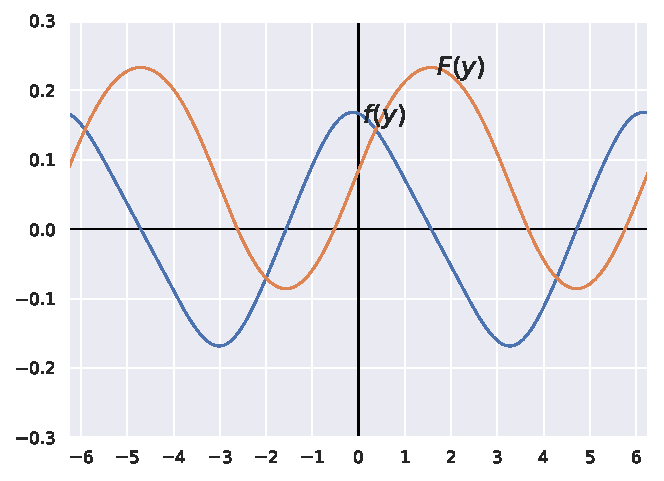
\includegraphics[width=0.7\linewidth]{graph_1}
	\label{fig:graph1}
\end{figure}

Let's see if we got the correct integral
by graphing it. One thing I've noticed
from this graph is that whenever $ f(y) $ is at $ 0 $, 
$ F(y) $ is either at its minimum or maximum.
For instance, at $ f(y) \approx -1.6 $,
$F(y)$ is at its minimum.
Notice that this is one of the properties we learned
in Calculus I. 

The integrand
of our original problem $ f(y) $ seems to be the
derivative of the integral we got, which is $ F(y) $.

\newpage

% ----------------------------- %
% Section 5
% ----------------------------- %
\section*{Analytically Verifying the Integral}

In fact, we know from the Fundamental Theorem of Calculus
that $ F'(x) = f(x) $.\footnote{
	Hass et al., \textit{Thomas' calculus} (14th ed.), Pearson, p. 280.
} This means we can analytically verify our integral by differentiating it. 
The derivative of our integral should be
the integrand of the original problem.
Let's use \textit{Maple} to
differentiate our integral: 
\begin{figure}
	\centering
	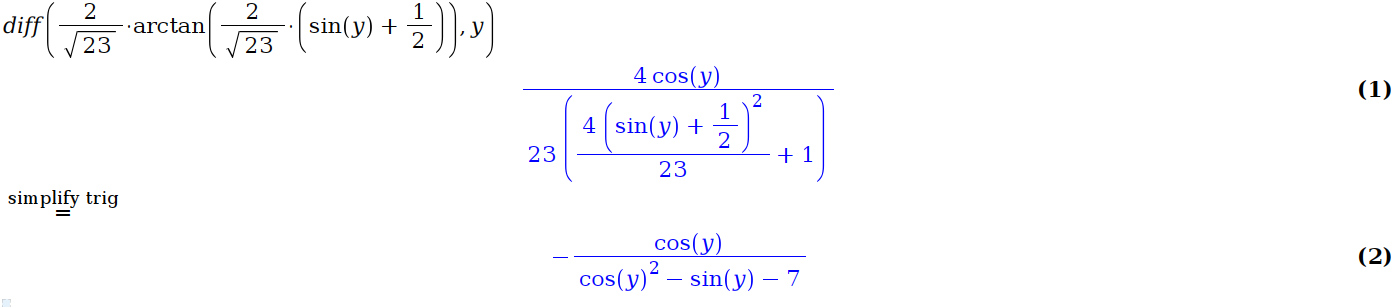
\includegraphics[width=0.98\linewidth]{maple}
	\caption{}
	\label{fig:maple}
\end{figure}

% ----------------------------- %
% Section 6
% ----------------------------- %
\section*{Conclusion}

The derivative of the integral indeed 
is equal to the integrand of the original problem. 
Therefore, we can finally conclude that the integral
we got is the correct integral:

\begin{equation*}
	\textbf{41.}\quad \int \frac{cosy}{sin^2y+siny-6} dy =	
	\frac{2}{\sqrt{23}} tan^{-1}\bigg(
	\frac{2}{\sqrt{23}}\big(
	siny+\frac{1}{2}
	\big)
	\bigg) + C
\end{equation*}

Plus, although we solved this problem
using u-substitution, completing the square,
and the integral of an $ arctan(x) $ function,
this problem comes from Chapter 8.5: 
\textit{Integration of Rational Functions
by Partial Fractions}, so keep in mind that
there must be another way of solving this problem by
using the partial fractions technique as well.

Thank you for your time, and I'll see you in two weeks
for AFP4!

% ----------------------------- %
% Section 7
% ----------------------------- %
\section*{Update}

June 30, 2022 - I've learned about partial fractions,
so now I know an alternative way to solve this problem, too.
\begin{flalign*}
	\textbf{41.}\quad \int \frac{cosy}{sin^2y+siny-6} dy 
	&= \int \frac{1}{u^2+u+6} du
	& & & (u = siny) \\[1ex]	
	&= \int \frac{\frac{1}{5}}{u-2} + 
	\frac{-\frac{1}{5}}{u+3} du
	& & & (\text{partial fraction decomposition}) \\[1ex]	
	&= \frac{1}{5}(ln|2-siny|-ln|3+siny|) + C
\end{flalign*}

Now, we've got a form different from
the first answer we got, which was in th form of
$ arctan(x) $, but plotting the first answer
and this answer on \textit{Maple} gives you
the same output. In other words, 
although in a different form, they are the same,
meaning that both answers are the correct integral.